\documentclass[12pt]{article}
\usepackage[dvipsnames]{xcolor}


\usepackage{../sty_files/packages}
\usepackage{../sty_files/shortcuts}
\usepackage{asymptote}

\setlist[itemize]{label=$\bullet$}
\setlength{\parindent}{0pt}

% \newcommand{\Newdot}{{\leavevmode\put(0,.63){\circle*{2.5}}}}
%--------------------------------------------------------------%
\begin{document}

\begin{titlepage}
   \begin{center}
       \vspace*{1cm}
       \textbf{\Huge {Trigs aren't Bad}}

       \vspace{1cm}
       \textbf{\Large{এস এম এ নাহিয়ান}}
       
       \vfill
       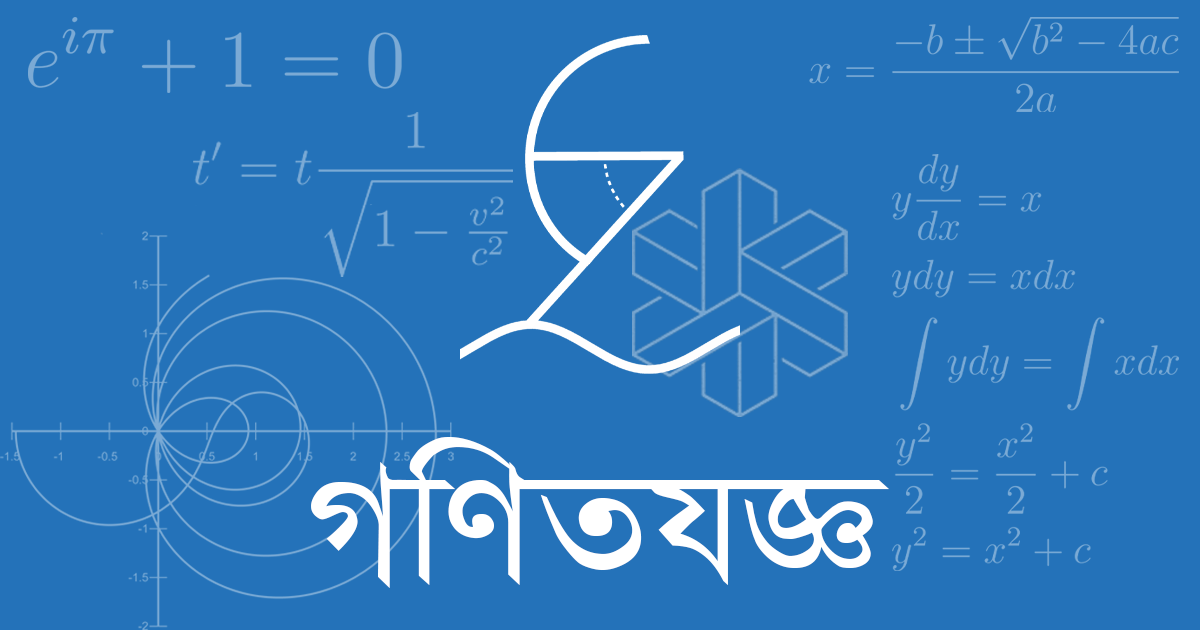
\includegraphics[width=0.4\textwidth]{images/meta.png}

       \large{গণিতযজ্ঞ}
   \end{center}
\end{titlepage}

\tableofcontents
%---------------------------------------------------------------%
\newpage
\section{Why to learn Trigonometry?}
ট্রিগ এমন একটি টুল যেটা দিয়ে সবসময় তুমি একটি প্রবলেম পুরোপুরি সমাধান করতে পারবে না। বরং সেটির 
একটা সাব-পার্ট এর জন্য ব্যাবহার করবে যেটা হয়তো সিন্থেটিক উপায়ে সলভ করতে গেলে অনেক বেশি সময় আর জটিল কন্সট্রাকশন 
এর দরকার পরবে। 
সাধারণত, তুমি চাইবে কন্টেস্ট টাইমে একটা প্রবলেম এর ছোট সাব-পার্ট এ কম সময় দিয়ে মূল সমস্যাতে বেশি ফোকাস করতে। \\
ন্যাশনাল লেভেল এর জিওমেট্রির জন্য ত্রিকোণোমিতি জানতেই হবে এমন কোনো বাধ্যবাধকতা নেই। বরং, প্রবলেম 
গুলো এমন ভাবেই বানানো হয় যেন শুধু ব্যাশিং করে সলভ করতে চাইলে সেটা সিন্থেটিক আপ্রোচ এর 
সমান অথবা আরো বেশি কঠিন হয়। কিন্তু তোমার যদি ত্রিকোণোমিতি আর সিন্থেটিক দুটিতেই ভালো এক্সপেরিয়েন্স থাকে 
তাহলে তুমি একটু বেশি এডভান্টেজ পাবে। কারণ, একটা বড় প্রবলেম সলভ করতে সেটার অনেক গুলো ছোটো 
পার্ট সলভ করতে হয়। সেখানে কিছু পার্ট সলভ করতে ত্রিকোণোমিতি বেশি সহজ হবে এবং কিছু পার্ট সলভ 
করতে সিন্থেটিক বেশি সহজ হবে।\\
তবে কখনো কখনো কিছু কঠিন প্রবলেমে ট্রিগ ব্যাবহার করলে সেটা এতো ট্রিভিয়াল হয়ে যায় যে মনে হয় 
ট্রিগ ব্যাবহার করা লিগ্যাল হওয়াই উচিত না :p। যেমন উদাহরণ হিসেবে রাফসান জানি\footnote[1]{https://www.facebook.com/raphsan.jani3011} ভাইয়ের একটা জিও দেখা যাক, 
\begin{exam} {উদাহরণ 1.1 (Raphsan Jani vai's কিউট জিও জিওঃ ৬৩৭)}
    মনে করি, সূক্ষ্মকোণী ত্রিভুজ $\triangle ABC$ এর অন্তবৃত্ত $BC, CA, AB$ কে যথাক্রমে $D, E, F$ বিন্দুতে স্পর্শ করে। ধরি, $\omega_A, 
    \omega_B, \omega_C$ বৃত্ত গুলো $BC, CA, AB$ কে যথাক্রমে $D, E, F$ বিন্দুতে স্পর্শ করে আর, 
    $BC, CA, AB$ ছোটো চাপ কে যথাক্রমে, $A', B', C'$ বিন্দুতে স্পর্শ করে।
    \begin{center}
        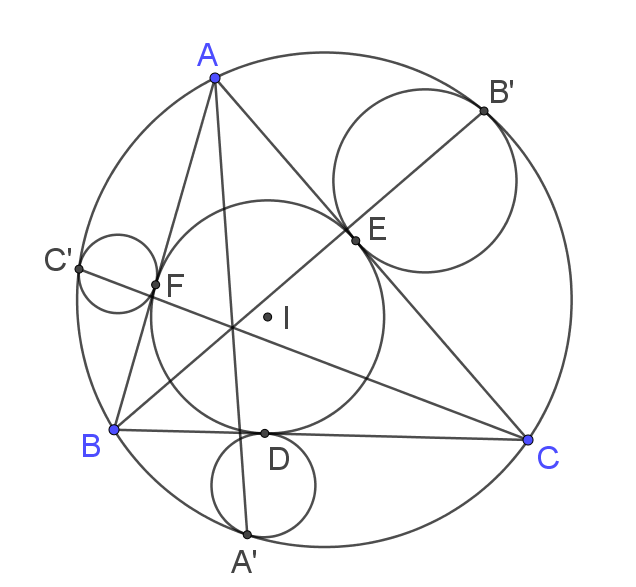
\includegraphics[width=0.5\textwidth]{images/JaniVaiProb.png}
    \end{center}
    প্রমাণ করো যে, $AA', BB', CC'$ সমবিন্দুগামী।
\end{exam} 
এই প্রবলেমটি আমরা ম্যাথ ক্যাম্প এ কয়েকজন মিলেও সিন্থেটিক ভাবে সমাধান করতে পারি নি। কিন্তু এই নোটে তোমরা 
পরে তোমরা দেখতে পাবে এটি কতো সহজে ট্রিগ ইউজ করে প্রমাণ করে ফেলা যায়। 
এছাড়াও কম্পিউটেশনাল জ্যামিতি তে প্রায়ই ট্রিগ ব্যাবহার করা অনেক হেল্পফুল হয়। যেমন, 
লেন্থ চেস, রেশিও রিলেটেড আপ্রোচ করতে গেলে অনেক ক্ষেত্রেই ত্রিকোণোমিতি ব্যাবহার করে সলভ করা সহজ হয়। \\

%% Example -----------------------------------------


\section{Some basic properties}
এই সেকশনটি কিছু ব্যাসিক ট্রিগ প্রোপার্টির একটি ছোটো রিভিশনের জন্য। যারা নিয়মিত ট্রিগ ব্যাবহার করো না তাদের 
পরবর্তি সেকশনে যাওয়ার আগে এই প্রোপার্টি গুলো জানা (ও ফিল করতে পারা) উচিত।
\begin{theom*}
    \begin{itemize}
        \item $\sin^2 \theta + \cos^2 \theta = 1$
        \item $\sin(-\theta) = -\sin\theta$
        \item $\cos(-\theta) = \cos\theta$
        \item $\sin(90\dg - \theta) = \cos\theta$
        \item $\cos(90\dg - \theta) = \sin\theta$
        \item $\sin(180\dg - \theta) = \sin\theta$
        \item $\cos(180\dg - \theta) = -\cos\theta$
        \item $\tan(90\dg - \theta) = \dfrac{1}{\tan\theta} = \cot \theta$
    \end{itemize}
\end{theom*}





\section{Theorems!!}
\subsection{Sine law}
ত্রিভুজ রিলেটেড প্রবলেম এ সবচেয়ে বেশি যে থিওরেম টি কাজে লাগে সেটি হলো Sine Law। এটি ত্রিভুজের বাহুর  
সাথে এর বিপরীত কোণের সম্পর্ক প্রকাশ করেস যেটি অনেক ইউজফুল। তো চলো আমরা Sine law এবং এর প্রমানটি দেখে ফেলি।
\begin{theom}{The Sine Law}
    কোনো ত্রিভুজ $ABC$ এর জন্য এর পরিব্যাসার্ধ $R$ এবং $BC = a, \ CA = b, \ AB = c$ হলে,
    $$ \dfrac{a}{\sin A} =  \dfrac{b}{\sin B} =  \dfrac{c}{\sin C} = 2R$$
\end{theom}
\begin{sol}
    \textbf{প্রমানঃ} ধরি $O$, $\triangle ABC$ এর পরিবৃত্তের কেন্দ্র। এবং $B'$, $O$ এর সাপেক্ষে $B$ এর রিফ্লেকশন।
    \begin{center}
        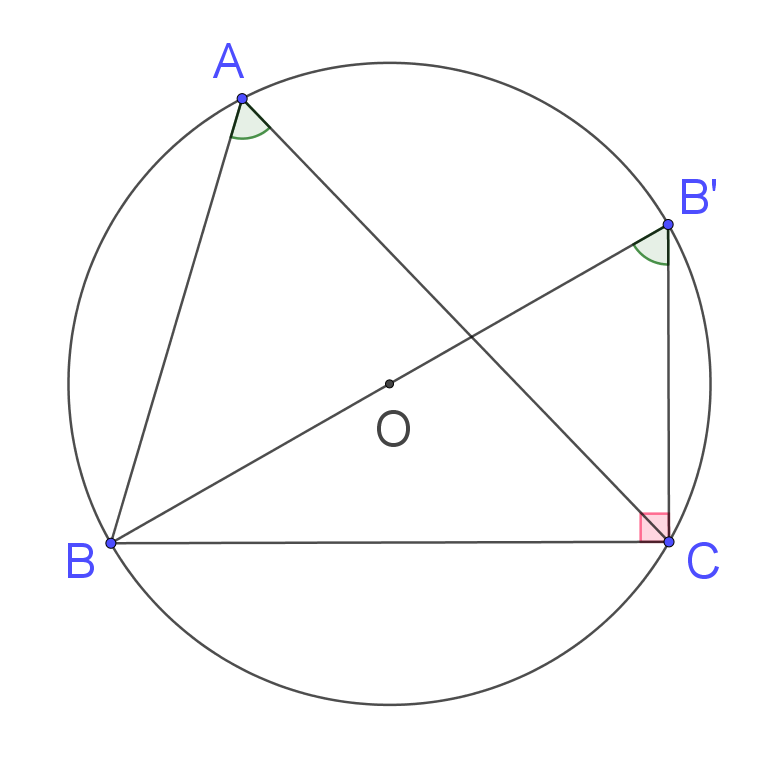
\includegraphics[width=.6\textwidth]{images/sine-law.png}\\
        চিত্রঃ Sine law
    \end{center}
    এখন, $BB'$ পরিবৃত্তের ব্যাস। সুতরাং, $\angle BCB' = 90\dg$। তাহলে,
    \begin{equation*}
        \sin(\angle BB'C) = \dfrac{BC}{BB'}\\
        \implies BB' = \dfrac{BC}{\sin(\angle BB'C)}\\
        \implies 2R = \dfrac{a}{\sin(\angle BAC)}
    \end{equation*}
    একইভাবে আমরা দেখাতে পারি, $$2R = \dfrac{b}{\sin B} =  \dfrac{c}{\sin C} \qed$$
\end{sol}


\subsection{Cosine law}
তোমরা সবাই পিথাগোরাস এর উপপাদ্যের সাথে পরিচিত। Cosine law মূলত সেটির ই এক্সটেন্ডেড ভার্শন। 
\begin{theom}{The Cosine law}
    কোনো ত্রিভুজ $ABC$ এ $BC = a, \ CA=b, \ AB = c$ হলে,
    $$c^2 = a^2 + b^2 - 2ab\cos C$$
\end{theom}
\begin{sol}
    \textbf{প্রমানঃ} প্রথমে $A$ থেকে $BC$ এর উপর $AH$ লম্ব আঁকি। ধরি, $AH=h$।
    \begin{center}
        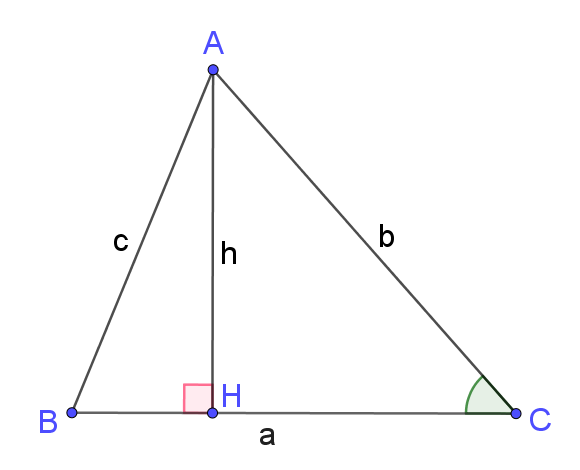
\includegraphics[width=.6\textwidth]{images/cosine-law.png}\\
        চিত্রঃ Cosine law
    \end{center}
    এখন,
    $$CH = AC\cos C =b\cos C \implies BH = BC-CH = a-b\cos C$$
    আবার, $$AH^2 = AC^2 - CH^2 = b^2 - b^2\cos^2 C$$ 
    দুটোকে মিলিয়ে পাই, \begin{align*}
        c^2 = AB^2 &= AH^2+BH^2\\
        &= b^2+b^2\cos^2 + (a-b\cos C)^2\\
        &= a^2+b^2 - 2ab\cos C \qed
    \end{align*}
\end{sol}


\subsection{Tangent law}
সাধারণত, Tangent law খুব একটা কাজে লাগে না। তবে জেনে রাখতে তো তো ক্ষতি নেই। 
\begin{theom}{The Tangent law}
    $ABC$ ত্রিভুজে, $BC = a, \ AC = b, \ \angle BAC = \alpha$ এবং $\angle ABC = \beta$ হলে,
    $${\displaystyle {\frac {a-b}{a+b}}={\frac {\tan {\tfrac {1}{2}}(\alpha -\beta )}{\tan {\tfrac {1}{2}}(\alpha +\beta )}}}$$
\end{theom}
\begin{sol}
    \textbf{প্রমানঃ} Sine law থেকে আমরা পাই, 
    $$\frac{a}{\sin \alpha} = \frac{b}{\sin \beta}$$
    $$\implies \frac{a}{b} = \frac{\sin \alpha}{\sin \beta}$$
    \begin{align*}
        \qquad \qquad \qquad \implies \frac{a-b}{a+b} &= \frac{\sin \alpha - \sin \beta}{\sin \alpha + \sin \beta}\\
        &= \frac{2\sin \tfrac {1}{2}(\alpha -\beta )\cos \tfrac {1}{2}(\alpha +\beta )}{2\sin \tfrac {1}{2}(\alpha +\beta )\cos \tfrac {1}{2}(\alpha -\beta )}\\
        &= \frac {\tan {\tfrac {1}{2}}(\alpha -\beta )}{\tan {\tfrac {1}{2}}(\alpha +\beta )} \qed
    \end{align*}
\end{sol}

\subsection{Trig Ceva} 
Sine law এর পর সম্ভবত Ceva's Theorem এর ত্রিকোণোমিতিক ভার্শন ই সবচেয়ে বেশি কাজে লাগে। 
\begin{theom}{Trigonometric version of Ceva's theorem}
    ধরি, $ABC$ ত্রিভুজে, $BC, CA, AB$ বাহুর উপর যথাক্রমে $D,E,F$ বিন্দু গুলো নেওয়া হলো। তাহলে, $AD, BE,CF$ 
    সমবিন্দুগামী হবে যদি এবং কেবল যদি, $$\dfrac{\sin\angle BAD \times\sin\angle ACF\times\sin\angle CBE}{\sin\angle CAD\times\sin\angle BCF\times\sin\angle ABE} = 1$$
\end{theom}
\begin{sol}
    \textbf{প্রমাণঃ} Ceva's theorem থেকে আমরা জানি, $AD, BE,CF$ সমবিন্দুগামী হবে যদি এবং কেবল যদি, 
    $\dfrac{BD\times AF\times CE}{CD\times BF\times AE} = 1$ হয়।
    \begin{center}
        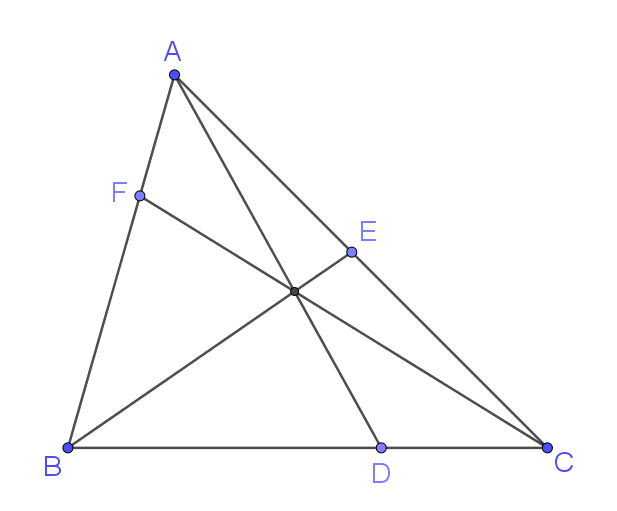
\includegraphics[width=0.6\textwidth]{images/trig-ceva.png}\\
        চিত্রঃ Ceva's theorem
    \end{center}
    এখন, $\triangle ABD$ তে Sine law ব্যাবহার করে পাই, $\dfrac{BD}{\sin\angle BAD} = 
    \dfrac{AD}{\sin B} \implies BD = \dfrac{AD\sin\angle BAD}{\sin B}$।\\
    একিভাবে আমরা $CD, BF, AF, AE,CE$ কেও প্রকাশ করতে পারবো। সুতরাং, 
    $$\dfrac{BD\times AF\times CE}{CD\times BF\times AE} = 1$$
    $$\iff \dfrac{\dfrac{AD\sin\angle BAD}{\sin B}\times \dfrac{CF\sin\angle ACF}{\sin A}\times \dfrac{BE\sin\angle CBE}{\sin C}}
    {\dfrac{AD\sin\angle CAD}{\sin C}\times \dfrac{CF\sin\angle BCF}{\sin B}\times \dfrac{BE\sin\angle ABE}{\sin A}} = 1$$
    $$\iff \dfrac{\sin\angle BAD \times\sin\angle ACF\times\sin\angle CBE}{\sin\angle CAD\times\sin\angle BCF\times\sin\angle ABE} = 1\qed$$
\end{sol}








\section{More Indentities}
কোনো সমস্যাতে ত্রিকোণোমিতি ব্যাবহারের সময় অনেক বীজগানিতিক ক্যালকুলেশন করতে হয়। তার জন্য কিছু 
আইডেন্টিটি জেনে রাখলে ট্রিগ ইকুয়েশন সলভ করতে সেগুলো কাজে লাগানো যায়। 
এই সেকশনে ত্রিকোণোমিতিক অনুপাত গুলোর যোগ ও গুনের কিছু আইডেন্টিটি দেখাবো।\\
এই আইডেন্টিটি গুলোর সাথে পরিচিত থাকলে এই সেকশনটি স্কিপ করতে পারো।\\
\subsection{Angle Sum and Difference}
প্রথমে আমরা দেখবো কোণের যোগ-বিয়োগের আইডেন্টিটি গুলো, 
\begin{theom*}
    যেকোনো দুটি কোণ, $\alpha$ ও $\beta$ এর জন্য,
    \begin{align*}
        \sin(\alpha +\beta )&=\sin \alpha \cos \beta +\cos \alpha \sin \beta \\
        \sin(\alpha -\beta )&=\sin \alpha \cos \beta -\cos \alpha \sin \beta \\
        \cos(\alpha +\beta )&=\cos \alpha \cos \beta -\sin \alpha \sin \beta \\
        \cos(\alpha -\beta )&=\cos \alpha \cos \beta +\sin \alpha \sin \beta 
    \end{align*}
\end{theom*}
\begin{sol}
    \textbf{প্রমাণ:} নিচের চিত্রে, $\sin(\alpha +\beta ) = \dfrac{DF}{AD}$ এবং 
    $\cos(\alpha +\beta ) = \dfrac{AF}{AD}$।
    \begin{center}
        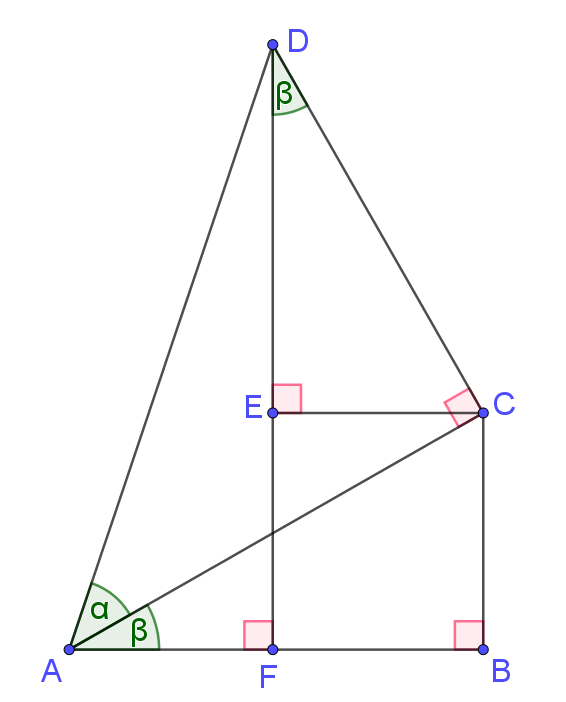
\includegraphics[width=.4\textwidth]{images/add-sine.png}\\
    \end{center}
    WLOG, ধরি, $AD = 1$। তাহলে, \begin{align*}
        \sin (\alpha + \beta)= FD &= FE+ED\\
        &= BC+CD\cos\beta\\
        &= AC\sin\beta + \sin\alpha\cos\beta\\
        &= \cos\alpha \sin\beta  +\sin\alpha\cos\beta \qed
    \end{align*}
    আবার, \begin{align*}
        \cos(\alpha +\beta ) &= AF = AB-FB\\
        &= AC\cos\beta - EC\\
        &= \cos\alpha+cos\beta - CD\sin\beta\\
        &=\cos \alpha \cos \beta -\sin \alpha \sin \beta \qed
    \end{align*}
\end{sol}
$\qquad$\\
এখন, বাকি দুটির প্রমান নিজে চেষ্টা করো।\\
হিন্টঃ $\sin(-\alpha) = -\sin\alpha, \ \cos(-\alpha) = \cos\alpha$\\

\subsection{Product to sum}
এবার আমরা দেখব ত্রিকোণোমিতিক অনুপাত গুলোর গুনফল থেকে যোগফল এ যাওয়ার কিছু আইডেন্টিটি।
\begin{theom*}
    যেকোনো দুটি কোণ, $\theta$ ও $\varphi$ এর জন্য,
    $${\displaystyle \cos \theta \cos \varphi =\dfrac{\cos(\theta -\varphi )+\cos(\theta +\varphi )}{2}}$$
    $${\displaystyle \sin \theta \sin \varphi =\dfrac{\cos(\theta -\varphi )-\cos(\theta +\varphi )}{2}}$$
    $${\displaystyle \sin \theta \cos \varphi =\dfrac{\sin(\theta +\varphi )+\sin(\theta -\varphi )}{2}}$$
    $${\displaystyle \cos \theta \sin \varphi =\dfrac{\sin(\theta +\varphi )-\sin(\theta -\varphi )}{2}}$$
\end{theom*}
$\qquad$\\
তোমরা হয়তো অলরেডি ধরে ফেলেছো যে এগুলো নতুন কিছুই নয়। ডানপক্ষে কোণের যোগ-বিয়োগের আইডেন্টিটি গুলো 
ব্যাবহার করলেই বামপক্ষ পেয়ে যাই আমরা। 
\subsection{Sum to product}
Product to sum এর আইডেন্টিটি গুলোকে এভাবে Sum to product হিসেবেও ব্যাবহার করা যায়, 
\begin{theom*}
    যেকোনো দুটি কোণ, $\theta$ ও $\varphi$ এর জন্য,
    $$\sin \theta + \sin \varphi =2\sin \left({\frac {\theta + \varphi }{2}}\right)\cos \left({\frac {\theta - \varphi }{2}}\right)$$
    $$\sin \theta - \sin \varphi =2\sin \left({\frac {\theta - \varphi }{2}}\right)\cos \left({\frac {\theta + \varphi }{2}}\right)$$
    $$\cos \theta +\cos \varphi =2\cos \left({\frac {\theta +\varphi }{2}}\right)\cos \left({\frac {\theta -\varphi }{2}}\right)$$
    $$\cos \theta -\cos \varphi =-2\sin \left({\frac {\theta +\varphi }{2}}\right)\sin \left({\frac {\theta -\varphi }{2}}\right)$$
\end{theom*}




% \subsection{Excercise}
% \begin{prob} {3.3.1}
%     প্রমাণ কর,
%     \begin{itemize}
%         \item $\tan(\alpha + \beta) = \dfrac{\tan\alpha + \tan\beta}{1- \tan\alpha\tan\beta}$
%         \item $\tan(\alpha - \beta) = \dfrac{\tan\alpha - \tan\beta}{1+ \tan\alpha\tan\beta}$
%     \end{itemize}
% \end{prob}
% \begin{prob} {3.3.2}
%     প্রমাণ কর, $\displaystyle \tan \theta \tan \varphi ={\frac {\cos(\theta -\varphi )-\cos(\theta +\varphi )}{\cos(\theta -\varphi )+\cos(\theta +\varphi )}}$\\
% \end{prob}
% \begin{prob} {3.3.2}
%     প্রমাণ করো, $\cos 20\dg \cos 40\dg \cos 80\dg = \frac{1}{8}$
% \end{prob}









\section{Trig ratios with triangle properties}
ত্রিকোণোমিতি ব্যাবহার করার (যেকোনো ধরনের ব্যাশিং এর ক্ষেত্রেই) সময় একটা কমন আপ্রোচ হলো কিছু ভ্যারিয়াবল 
ডিফাইন করা (সাধারণত Degree of freedom সংখ্যক) এবং সেগুলো ব্যাবহার করে বাকি সব কিছুর মান বের করার চেষ্টা করা।\\
এক্ষেত্রে তুমি স্বাভাবিক ভাবেই চাইবে ত্রিভুজ রিলেটেড প্রবলেমে সেটির কোণ গুলোর ত্রিকোণোমিতিক অনুপাত গুলোর মানকে 
সেটির বাহুর ভ্যারিয়াবল গুলো দিয়ে প্রকাশ করতে। \\
এভাবে কোনো কোণের Cos অনুপাত বের করা খুবই সহজ। Cosine law থেকেই আমরা পেয়ে যাই, 
\begin{theom*}
    $$\cos A= \dfrac{b^2+c^2-a^2}{2bc}$$
\end{theom*}
$\qquad$\\
এখান থেকে আমরা পিথাগোরাসের ত্রিকোণোমিতিক আইডেন্টিটি ব্যাবহার করে পাই, \begin{align*}
    \sin A &= \sqrt{1-\dfrac{(b^2+c^2-a^2)^2}{(2bc)^2}}\\
    &= \dfrac{\sqrt{(2bc)^2 - (b^2+c^2-a^2)^2}}{2bc}\\
    &= \dfrac{\sqrt{(2bc +b^2+c^2-a^2)((2bc -b^2-c^2+a^2))}}{2bc}\\
    &= \dfrac{\sqrt{\{(b+c)^2-a^2\}\{(a^2-(b-c)^2)\}}}{2bc}\\
    &= \dfrac{\sqrt{(a+b+c)(-a+b+c)(a-b+c)(a+b-c)}}{2bc}\\
\end{align*}
এখান থেকে ত্রিভুজের অর্ধ-পরিসীমাকে $s = \dfrac{a+b+c}{2}$ ধরে মান বসিয়ে আমরা পেয়ে যাই, 
\begin{theom*}
    $$\sin A = \dfrac{2\sqrt{s(s-a)(s-b)(s-c)}}{bc}$$
\end{theom*}
$\qquad$\\
তোমরা হয়তো ভাবতে পারো আমি কেনো $a,b,c$ বাদ দিয়ে $s-a, s-b, s-c$ এর মাধ্যমে প্রকাশ করতে যাব।\\
কিন্তু তোমরা খেয়াল করলেই ইনসেন্ট্রিক ডায়াগ্রামে এই দৈর্ঘ্যের রেখাংশ খুজে পাবে।
\begin{center}
    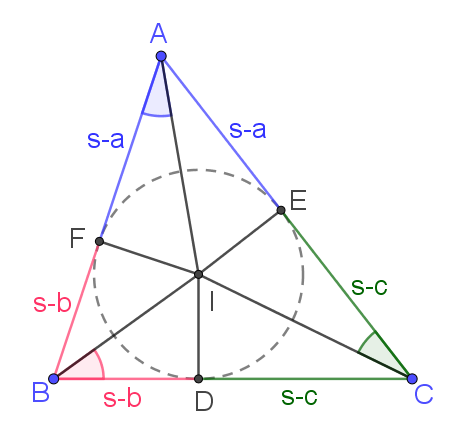
\includegraphics[width=0.6\textwidth]{images/incircle.png}\\
    চিত্রঃ ইনসেন্ট্রিক ডায়াগ্রামে
\end{center}
এই ডায়াগ্রাম থেকে এখন আমরা $\frac12 \angle A$ এর ত্রিকোণোমিতিক অনুপাত গুলো ও বের করতে পারি, \\
আমরা জানি, ত্রিভুজের ক্ষেত্রফল $=\sqrt{s(s-a)(s-b)(s-c)}$ আবার, $$\area (ABC) = \area(ABI)+\area(BCI)+\area(CAI)$$
$$\implies \sqrt{s(s-a)(s-b)(s-c)} = \dfrac{1}{2} r(a+b+c) = rs$$
$$\implies r = \sqrt{\dfrac{(s-a)(s-b)(s-c)}{s}}$$
এখানে $r$ হলো অন্তবৃত্তের ব্যাসার্ধ। পিথাগোরাসের উপপাদ্য ব্যাবহার করে আমরা পেয়ে যাই,
\begin{align*}
    AI &= \sqrt{(s-a)^2 + \dfrac{(s-a)(s-b)(s-c)}{s}}\\
    &= \sqrt{(s-a)\dfrac{s(s-a)+(s-b)(s-c)}{s}}\\
    &= \sqrt{(s-a)\dfrac{s^2 - sa + s^2 - sb- sc+bc}{s}}\\
    &= \sqrt{(s-a)\dfrac{2s^2 - s(a+b+c)+bc}{s}}\\
    &= \sqrt{(s-a)\dfrac{2s^2 - 2s^2+bc}{s}} = \sqrt{(s-a)\dfrac{bc}{s}}\\
\end{align*}
এবার এই মান গুলো $\triangle AIF$ এর সাথে ব্যাবহার করে কিছু অ্যালজেব্রিক ক্যাল্কুলেশন করেই 
পেয়ে যাই,
\begin{theom*}
    $$\sin \frac A2 = \sqrt{\dfrac{(s-b)(s-c)}{bc}} \text{ এবং } 
    \cos\frac A2 = \sqrt{\dfrac{s(s-a)}{bc}}$$
\end{theom*}
এখন আবার, \begin{align*}
    \sin A &= 2\sin\dfrac A2 \cos\dfrac A2\\
    \implies \sin A &= 2\sqrt{\dfrac{(s-b)(s-c)}{bc}} \cdot \sqrt{\dfrac{s(s-a)}{bc}}\\
    \implies \sin A &= 2\sqrt{\dfrac{(s-b)(s-c)s(s-a)}{bc^2}}\\
    \implies \dfrac 1 2 bc\sin A &= \sqrt{(s-b)(s-c)s(s-a)}\\
\end{align*}
$\qquad$\\
এবং আমরা ত্রিভুজের ক্ষেত্রফলকে ত্রিকোণোমিতিক অনুপাতের সাহায্যে প্রকাশ করতে পারি,
\begin{theom*}
    $$\area(ABC) = \dfrac 12 ab\sin C = \dfrac 12 bc\sin A = \dfrac 12 ca\sin B$$
\end{theom*}


\section{Other cool facts and identities}
এই সেকশনে কিছু র‍্যান্ডম ফ্যাক্ট ও আইডেন্টিটি দেখানো হবে। এই ফ্যাক্ট গুলো আমাদের খুব বেশি কাজে আসবে না। 
কিন্তু এগুলো আমাদের কিছু আইডিয়া শেখাবে যা সমস্যা সমাধানের জন্য কাজে লাগতে পারে। আর এই ফ্যাক্ট গুলোর 
কিছু কিছুর প্রমাণ এই নোটের স্কোপের বাইরে তাই সেগুলো আমি এখানে দেখাচ্ছি না।\\
ট্রিগ এ একদম বিগিনারদের এই সেকশনটি স্কিপ করতে পারো। 
\subsection{Double, tripple angles}
কোণের যোগ-বিয়োগের আইডেন্টিটি ব্যাবহার করে $2A, 3A$ এসব কোণের ত্রিকোণোমিতিক অনুপাত গুলো পাওয়া যায়, 
\begin{itemize}
    \item $\sin 2A = 2\sin A \cos A =(\sin A +\cos A )^{2}-1$
    \item $\cos 2A = \cos^2 A - \sin^2 A = 2\cos^2 A - 1 = 1- 2\sin^2A$
    \item $\sin 3A = 3\sin A - 4\sin^3 A$
    \item $\cos 3A = 4\cos^3 A - 3\cos A$
\end{itemize}
এগুলো থেকে পক্ষান্তর করে পাওয়া যায়, 
\begin{itemize}
    \item ${\displaystyle \sin ^{2}\theta ={\frac {1-\cos(2\theta )}{2}}}$
    \item ${\displaystyle \cos ^{2}\theta ={\frac {1+\cos(2\theta )}{2}}}$
    \item ${\displaystyle \sin ^{3}\theta ={\frac {3\sin \theta -\sin(3\theta )}{4}}}$
    \item ${\displaystyle \cos ^{3}\theta ={\frac {3\cos \theta +\cos(3\theta )}{4}}}$
\end{itemize}
\subsection{Values for special angles}
স্পেশাল কোণের ট্রিগ অনুপাত থেকে জন্য কিছু কুল মান পাওয়া যায়, (যদিও খুব একটা কাজের না)
\begin{itemize}
    \item ${\displaystyle \cos 20^{\circ }\cdot \cos 40^{\circ }\cdot \cos 80^{\circ }={\frac {1}{8}}}$
    \item ${\displaystyle {\sin 15^{\circ }\cdot \sin 45^{\circ }\cdot \sin 75^{\circ }={\frac {\sqrt {2}}{8}}}}$
    \item ${\displaystyle \sin 20^{\circ }\cdot \sin 40^{\circ }\cdot \sin 80^{\circ }={\frac {\sqrt {3}}{8}}}$
    \item $\sin 15^{\circ }\cdot \sin 75^{\circ } ={\dfrac {1}{4}}$
\end{itemize}
\subsection{Identities for triangle angles}
ত্রিভুজের তিনটি কোণ $ \displaystyle \alpha +\beta +\gamma =180^{\circ }$ হলে, 
\begin{itemize}
    \item $\tan\alpha + \tan\beta + \tan\gamma = \tan\alpha \tan\beta \tan\gamma$
    \item $\sin\alpha + \sin\beta + \sin\gamma = 4\cos \left(\dfrac{\alpha}{2} \right)\cos \left(\dfrac{\beta}{2} \right)\cos \left(\dfrac{\gamma}{2} \right)$
    \item $\sin 2\alpha + \sin 2\beta + \sin 2\gamma = 4\cos \alpha \cos \beta \cos \gamma$
\end{itemize}
\subsection{Long sequence product}
কিছু ট্রিগ সিকুয়েন্স এর সুন্দর গুনফল পাওয়া যায়। এগুলো আমি কখনো জিও প্রবলেমে ব্যাবহার হতে দেখি নি কিন্তু 
বীজগনিতের কিছু প্রবলেম এ এগুলোর ক্লেভার ব্যাবহার দেখেছি,
\begin{itemize}
    \item ${\displaystyle \prod _{j=0}^{k-1}\cos \left(2^{j}x\right)={\frac {\sin \left(2^{k}x\right)}{2^{k}\sin x}}}$
    \item ${\displaystyle \prod _{k=1}^{n-1}\sin \left({\frac {k\pi }{n}}\right)={\frac {n}{2^{n-1}}}.}$
\end{itemize}






\section{Examples}
\begin{exam} {উদাহরণ 7.1 (Raphsan Jani vai's কিউট জিও জিওঃ ৬৩৭)}
    মনে করি, সূক্ষ্মকোণী ত্রিভুজ $\triangle ABC$ এর অন্তবৃত্ত $BC, CA, AB$ কে যথাক্রমে $D, E, F$ বিন্দুতে স্পর্শ করে। ধরি, $\omega_A, 
    \omega_B, \omega_C$ বৃত্ত গুলো $BC, CA, AB$ কে যথাক্রমে $D, E, F$ বিন্দুতে স্পর্শ করে আর, 
    $BC, CA, AB$ ছোটো চাপ কে যথাক্রমে, $A', B', C'$ বিন্দুতে স্পর্শ করে।\\
    প্রমাণ করো যে, $AA', BB', CC'$ সমবিন্দুগামী।
\end{exam} 
\begin{sol}
    \textbf{সমাধানঃ} মনে করি, $BAC$ চাপের মধ্যবিন্দু $X$। আমরা জানি, $A,D,X$ সমবিন্দুগামী। 
    \begin{center}
        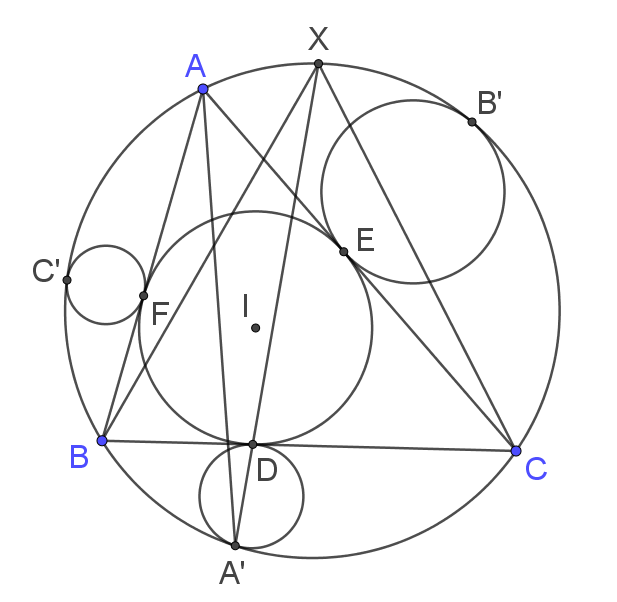
\includegraphics[width = 0.5\textwidth]{images/JaniVaiSol.png}
    \end{center}
    এখন, $\triangle XBD$ তে Sine law ব্যাবহার করে পাই, 
    $$\sin BAA' = \sin BXA' = \sin BXD = \dfrac{BD \sin XBC}{XD}$$
    একইভাবে, $\sin CAA' = \dfrac{CD \sin XCB}{XD}$। তাহলে, 
    $$\dfrac{\sin BAA'}{\sin CAA'} = \dfrac{\dfrac{BD \sin XBC}{XD}}{\dfrac{CD \sin XCB}{XD}} = \dfrac{BD}{CD}$$
    একইভাবে, $\dfrac{\sin ACC'}{\sin BCC'} = \dfrac{AF}{BF}$, $\dfrac{\sin CBB'}{\sin ABB'} = \dfrac{CE}{AE}$।
    এবং এগুলোকে গুন করলেই আমরা পেয়ে যাই যে Ceva's theorem এর কন্ডিশন সত্য। সুতরাং $AA', BB', CC'$ সমবিন্দুগামী। $\qed$
\end{sol}

\begin{exam} {উদাহরণ 7.2}
    \begin{center}
        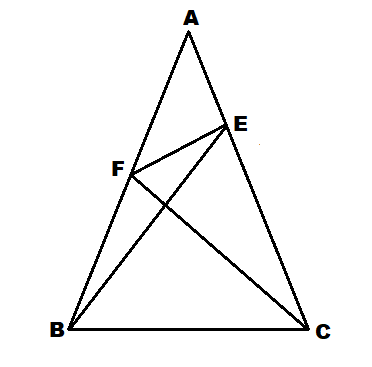
\includegraphics[width=0.35\textwidth]{images/gz-exmple.png}
    \end{center}
    যদি $AB=AC$, $\angle ABE=20°$, $\angle EBC=60°$, $\angle ACF=30°$, $\angle FCB=50°$ হয়, তাহলে $\angle FEB = ?$
\end{exam}
\begin{sol}
    \textbf{সমাধানঃ} প্রথমেই, $\angle BFC = 50\dg, \angle BEC = 40\dg$। ধরি, $\angle FEB = x$। তাহলে, $\angle CFE = 110\dg - x$। \\
    এখন, $\triangle  FEB, \triangle FCB, triangle BEC, \triangle FEC$ তে Sine law ব্যাবহার করে পাই,
    \begin{align*}
        FE &= \dfrac{BF \sin 20\dg}{\sin x} \\
        BF &= \dfrac{BC \sin 50\dg}{\sin 50\dg} = BC \\
        BC &= \dfrac{CE \sin 40\dg}{\sin 60\dg} \\
        CE &= \dfrac{FE \sin 110\dg - x}{\sin 30\dg} \\
    \end{align*}
    এখন মান গুলো বসিয়ে পাই, 
    \begin{align*}
        &FE = \dfrac{FE \sin 20\dg \sin 40\dg \sin (110\dg - x)}{\sin x \sin 60\dg\sin 30\dg}\\
        \implies & \sin 20\dg \sin 40\dg \sin (110\dg - x) = \sin x \sin 60\dg\sin 30\dg\\
        \implies &\sin 20\dg \sin 40\dg \cos(x-20\dg)\sin 80\dg = \sin x \sin 60\dg\sin 30\dg \sin 80\dg\\
        \implies & \dfrac{\sqrt 3}{8} \cos(x-20\dg) = \dfrac{\sqrt 3}{4}\sin x \sin 80\dg \text{[Well known]}\\
        \implies & \cos(x-20\dg) = 2\sin x \sin 80\dg\\
        \implies & \cos x \cos 20\dg + \sin x \sin 20\dg = 2\sin x \sin 80\dg\\
        \implies & \cos x = \dfrac{2\sin x \sin 80\dg - \sin x \sin 20\dg}{\cos 20\dg}\\
        \implies & \dfrac{\cos x}{\sin x} = \dfrac{\sin 80\dg + \sin 80\dg - \sin 20\dg}{\cos 20\dg}\\
        \implies & \dfrac{\cos x}{\sin x} = \dfrac{\sin 80\dg + 2\sin \left( \dfrac{80\dg - 20\dg}{2} \right)\cos\left(\dfrac{80\dg + 20\dg}{2}\right)}{\cos 20\dg}\\
        \implies & \dfrac{\cos x}{\sin x} = \dfrac{\sin 80\dg + \cos\left(50\dg\right)}{\cos 20\dg}\\
        \implies & \dfrac{\cos x}{\sin x} = \dfrac{\sin 80\dg + \sin\left(40\dg\right)}{\cos 20\dg}\\
        \implies & \dfrac{\cos x}{\sin x} = \dfrac{2\sin \left( \dfrac{80\dg + 40\dg}{2} \right)\cos\left(\dfrac{80\dg - 40\dg}{2}\right)}{\cos 20\dg}\\
        \implies & \dfrac{\cos x}{\sin x} = \dfrac{2\sin \left( 60\dg \right)\cos\left(20\dg\right)}{\cos 20\dg}\\
        \implies & \dfrac{\cos x}{\sin x} =\sqrt 3\\
    \end{align*}
    সুতরাং, $x = 30\dg$ কারণ, $x < 180\dg \ \qed$
\end{sol}

\begin{exam} {উদাহরণ 7.3}
    ত্রিভুজ $ABC$ তে $\angle B > 45\dg, \ \angle C > 45\dg$। $AC$ ও $AB$ বাহুর উপর ত্রিভুজটির 
    বাইরে দুটি সমকোণী সমদ্বিবাহু ত্রিভুজ $CAM, BAN$ আকা হলো যেনো, $AB=AN$ ও $AC = AM$ হয়। 
    এরপর ত্রিভুজটির ভিতর $P$ একটি বিন্দু নেই যেনো, $PB=PC$ এবং 
    $\angle BPC = 90\dg$ হয়।\\
    প্রমাণ করো যে, $\angle MPN = 90\dg$।
\end{exam}
\begin{sol}
    \textbf{সমাধানঃ} এখানে, $\angle PBC = \angle NBA = 45\dg$ সুতরাং, $\angle PBN = \angle B$।\\
    একইভাবে, $\angle PCN = \angle C$।\\
    ধরি, $BC = a, \ CA = b,\ AB = c$।\\
    তাহলে, $AM = b,\ AN = c$ এবং $BP = PC = \dfrac{a}{\sqrt 2}$ [$\sin 45\dg$ ব্যাবহার করে]।\\
    এখন, $\triangle ABC$ তে Cosine law ব্যাবহার করে পাই, 
    \begin{align*}
        a^2 &= b^2 + c^2 - 2bc\cos A \qquad(1)\\
        b^2 &= a^2 + c^2 - 2ac\cos B \qquad(2)\\
        c^2 &= a^2 + b^2 - 2ab\cos C \qquad(3)
    \end{align*}
    \begin{center}
        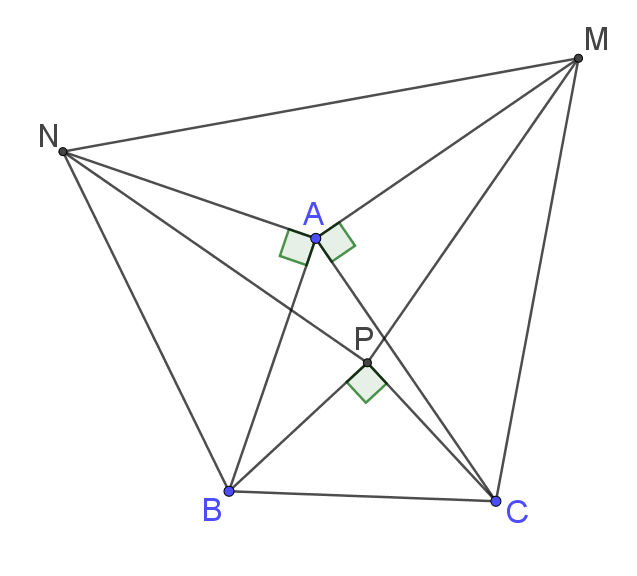
\includegraphics[width=0.6\textwidth]{images/symtry.png  }
    \end{center}
    আবার, $\triangle PCM, \ \triangle PBN$ ও $\triangle AMN$ এ Cosine law ব্যাবহার করে পাই, 
    \begin{align*}
        PM^2 &= \frac{a^2}{2} + 2b^2 - 2ab\cos C \qquad(4)\\
        PN^2 &= \frac{a^2}{2} + 2c^2 - 2ac\cos B \qquad(5)\\
        MN^2 &= b^2 + c^2 - 2bc\cos MAN\\
        &= b^2 + c^2 - 2bc\cos (180\dg - A)\\
        &= b^2 + c^2 + 2bc\cos A  \qquad(6)
    \end{align*}
    তাহলে, 
    \begin{align*}
        PM^2 + PN^2 &= a^2 + 2b^2 + 2c^2 - 2ab\cos C - 2ac\cos B\\
        &= a^2 + 2b^2 + 2c^2 + (c^2 - a^2 - b^2) + (b^2 - a^2 - c^2) \ [\text{(2) ও (3) হতে}] \\
        &= 2b^2 + 2c^2 - a^2\\
        &= 2b^2 + 2c^2 - (b^2 + c^2 - 2ab\cos A) \ [\text{(1) হতে}]\\
        &= b^2 + c^2 + 2ab\cos A\\
        &= MN^2 \ [\text{(6) হতে}]
    \end{align*}
    সুতরাং পিথাগোরাসের বিপরীত উপপাদ্য ব্যাবহার করে পাই $\angle MPN = 90\dg$ $\qed$
\end{sol}

% \begin{exam} {উদাহরণ (BdMO 2021 Divitional Secondary P8)}
%     চিত্রে, $AB$ ও $AC$ যথাক্রমে $5$ একক ব্যাসার্ধের $O$ এবং $O'$ কেন্দ্র বিশিষ্ট বৃত্তের বৃত্তচাপ। 
%     $OO' = 6$ একক। $\triangle ABC$ এ $AB = AC$ এবং ত্রিভুজের ভিতর একটি বৃত্ত অন্তঃস্পর্শ করে 
%     আছে। বৃত্তের ব্যাসার্ধকে $r = \dfrac{a}{\sqrt{b+1}}$ আকারে লেখা যায়, যেখানে $a,b$ পূর্ণ সংখ্যা। $a+b=?$ 
%     \begin{center}
%         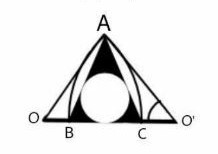
\includegraphics[width=0.5\textwidth]{images/divitional.jpeg}
%     \end{center}
% \end{exam}
% \begin{sol}
    
% \end{sol}
% \begin{exam} {উদাহরণ}
    
% \end{exam}
% \begin{sol}
    
% \end{sol}
\begin{exam} {উদাহরণ 7.4}
    মনে করি $ABC$ ত্রিভুজে $BC$ সবচেয়ে লম্বা বাহু। ধরি $O$, $ABC$ এর বহিকেন্দ্র। $P$, $BC$ বাহুর উপর 
    যেকোনো একটি বিন্দু। $BP$ এর লম্ব সমদ্বিখণ্ডক $AB$ কে $Q$ বিন্দুতে এবং $CP$ এর লম্ব সমদ্বিখণ্ডক $AC$ কে $R$ বিন্দুতে ছেদ করো। প্রমাণ করো যে, $AQOR$ একটি বৃত্তস্থ চতুর্ভুজ।
\end{exam}
\begin{sol}
    \textbf{সমাধানঃ} মনে করি, $M, N$ যথাক্রমে $AB, AC$ এর মধ্যবিন্দু। তাহলে, $\angle OMQ = \angle ONR = 90\dg$ এবং $AMON$ বৃত্তস্ত। \\
    এখন ধরি, $Q$, $AM$ রেখাংশের ভেতর অবস্থিত [অন্য কে্সেও আমরা একই ভাবে প্রমাণ করতে পারব]। তাহলে, $R$, $CN$ 
    রেখাংশের ভেতর থাকবে।\\
    এখন, $A,Q, O, R$ বৃত্তস্থ প্রমাণ করতে হলে, $\angle OQM = \angle ORN$ বা $\triangle OQM \sim \triangle ORN$ হতে হবে।\\
    \begin{center}
        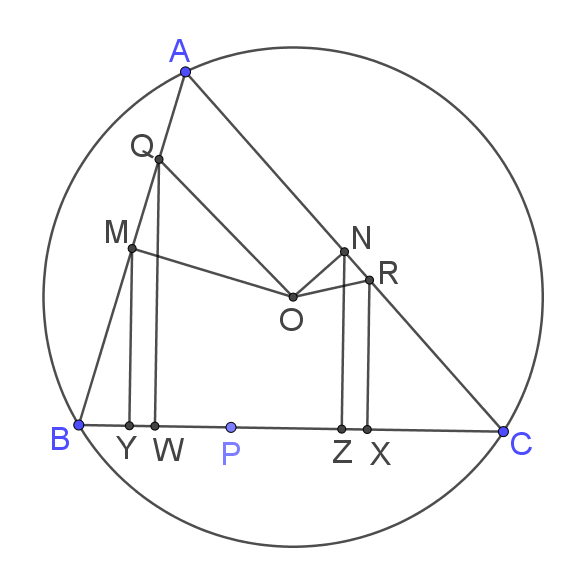
\includegraphics[width = 0.6\textwidth]{images/camptest.png}
    \end{center}
    আমরা জানি, $\angle OAN = 90\dg - \angle B$ এবং $\angle OAM = 90\dg - \angle C$। তাহলে, $\triangle MON$ এ Sine law ব্যাবহার করে পাই,
    \begin{align*}
        &\dfrac{OM}{\sin ONM} = \dfrac{ON}{\sin OMN}\\
        \implies &\dfrac{ON}{OM} = \dfrac{\sin OMN}{\sin ONM}\\
        \implies &\dfrac{ON}{OM} = \dfrac{\sin OAN}{\sin OAM}\\
        \implies &\dfrac{ON}{OM} = \dfrac{\sin (90\dg - \angle B)}{\sin (90\dg - \angle C)}\\
        \implies &\dfrac{ON}{OM} = \dfrac{\cos  B}{\cos  C} \qquad(1)\\
    \end{align*}
    ধরি, $PB$ ও $PC$ এর মধ্যবিন্দু যথাক্রমে $W$, $X$। এবং $M$ ও $N$ থেকে $BC$ এর উপর লম্বের পাদবিন্দু যথাক্রমে $Y$ ও $Z$। \\
    এখন, $WX = WP+XP = \dfrac 12 (BP+CP) = \dfrac 12 BC$ এবং $YZ = MN = \dfrac 12 BC$।\\
    সুতরাং, $WX = YZ$। তাহলে, $WY = XZ = x$ [ধরি, $WY= x$]\\
    এখন, $$\cos B = \dfrac{BW}{BQ} = \dfrac{BY}{BM} = \dfrac{BY-BW}{BM-BQ} = \dfrac{WY}{QM} =\dfrac{x}{QM}$$
    একইভাবে, $$\cos C = \dfrac{x}{RN}$$
    সুতরাং, $(1)$ এ মান বসিয়ে পাই,
    $$\dfrac{ON}{OM} = \dfrac{\cos  B}{\cos C} = \dfrac{\frac{x}{QM}}{\frac{x}{RN}} = \dfrac{RN}{QM}$$
    তাহলে আমরা পাই, $\triangle OQM \sim \triangle ORN$ যেটা আমরা প্রমাণ করতে চেয়েছিলাম। $\qed$
\end{sol}

\section{Some motivations about when/how to use?} % May delete this
এই সেকশনে বলা কেস/উপায় গুলোই একমাত্র নয় এগুলো ছাড়াও আরো অনেক কেস/উপায় এ ট্রিগ ব্যাবহার করা সম্ভব। \\
এখানে আমি কিছু কমন কেস এর কথা বলব যেগুলোতে বেশিরভাগ সময়েই সিন্থেটিক ভাবে চেষ্টা করার চেয়ে ট্রিগ ব্যাবহার করা সহজ হবে।\\
\begin{itemize}
    \item কম্পিউটেশনাল প্রবলেম স্টেটমেন্টে অনেক সুন্দর সুন্দর কোণ ($15\dg,30\dg, 
        45\dg,60\dg, 75\dg$) থাকলে সেগুলোর ত্রিকোণোমিতিক অনুপাত নিয়ে গুতোগুতি করতে পারো।
    \item ব্যাকট্র্যাকিং করে অনেক সমান অনুপাতের রেখাংশ পেলে কিন্তু সেগুলো স্বাভাবিক ভাবে কোনো 
        সদৃশ ত্রিভুজ গঠন না করলে (সদৃশ ত্রিভুজ পেলে সিন্থেটিক ভাবেই চেষ্টা করা বেটার)।
    \item যদি দেখো যে প্রয়োজনীয় সব দৈর্ঘ্যকে ত্রিভুজের বাহুর দৈর্ঘ্য দিয়ে সহজে প্রকাশ করা যাচ্ছে এবং 
        যা প্রমান করতে বলা হয়েছে সেটিও দৈর্ঘ্য রিলেটেড।
    \item কনকারেন্সি রিলেটেড প্রবলেম এ ত্রিভুজের সেভিয়ান পাওয়া গেলে এবং কোণ গুলোর $\sin$ কে ব্যাবহার করা গেলে।
    \item অনেক বেশি সমকোণী ত্রিভুজ থাকলে এবং তাদের বাকি কোণ গুলোর প্রোপার্টি জানা থাকলে।
    \item একাধিক বৃত্তে সমান কোণের জ্যা থাকলে।
\end{itemize}


\section{Common (?) Mistakes}
এই সেকশনে আমি কিছু ভুল দেখাবো যেগুলো বিগিনার রা অনেক ক্ষেত্রেই করে থাকে (এখানকার কিছু ভুল 
আমার নিজের থেকেই নেওয়া)। 
\begin{itemize}
    \item $\sin \alpha = \sin \beta \implies \alpha = \beta$
    \begin{description}
        \item[Explanation:] এটা খুবই কমন একটা মিস্টেক। এটার কাউন্টার এক্সাম্পল টা 
        জেনেও অনেকে এই ভুল টা করে। $\beta = 180\dg - \alpha$ 
        হলেও $\sin \alpha = \sin \beta$ হয়।
    \end{description}
    \item $\dfrac{\sin\angle BAX}{\sin\angle CAX} = \dfrac{\sin\angle BAY}{\sin\angle CAY}
        \implies A, X$ এবং $Y$ সমরেখ। 
    \begin{description}
        \item[Explanation:] এই ভুল টা আমি নিজেও করেছিলাম। বিগিনারদের কাছে এটা কিছুটা 
            ইন্টুইটিভ লাগতে পারে। বাট এটার সবচেয়ে সহজ কাউন্টার এক্সাম্পল টা খুবই ডিসরেস্পেক্টফুল।\\
            $A, B, C$ সমরেখ হলে \textbf{যেকোনো}, $X,Y$ এর জন্যই এটা সত্য হয় কেননা 
            দুই পাশেই সবসময় $1$ হবে সেক্ষেত্রে। :) এখন যারা ভাবছো, তাহলে $A, B, C$ সমরেখ না হলে 
            হয়তো এটা সত্যি হবে। তাদের জন্য নেক্সট ভুল টা।
    \end{description}
    \item $\dfrac{\sin\angle BAX}{\sin\angle CAX} = \dfrac{\sin\angle BAY}{\sin\angle CAY}$ 
        এবং $A, B, C$ সমরেখ না হলে $A, X$ এবং $Y$ সমরেখ। 
    \begin{description}
        \item[Explanation:] This feels so intuitive. বাট এটাও সত্যি না :") 
            তবে এক্ষেত্রে তুমি এটা বলতে পারবে যে, হয়, $A, X$ এবং $Y$ সমরেখ অথবা,
            $A(B,C;X,Y) = -1$। এটা প্রোজেক্টিভ জিওমেট্রির একটা নোটেশন। তাই না জানলেও 
            ক্ষতি নেই।
    \end{description}
\end{itemize}



\section{Practice problems}
\begin{prob} {10.1 (Raphsan Jani vai's কিউট জিও জিওঃ ৩৪৯)}
    $\triangle ABC$ তে $AC = BC$ এবং $\angle ACB = 20\dg$। $D$, $BC$ এর উপর একটি বিন্দু যেনো, 
    $\angle CAD = 10\dg$ হয়। প্রমাণ কর যে, $AB = CD$। 
\end{prob}

\begin{prob} {10.2}
    $ABCD$ সামান্তরিকে $\angle A$ সূক্ষ্মকোণ। $P$, সামান্তরিকের বাইরে একটি বিন্দু যেনো, $\angle PBC = \angle PDC$ হয়।
    প্রমাণ কর যে, $\angle PAB + \angle PCB = 180\dg$।
\end{prob}

\begin{prob} {10.3 (BdMO 2016 National Secondary P2)}
    ত্রিভুজ $\triangle ABC$ সমদ্বিবাহু এবং $AB=AC$। $P$, $\triangle ABC$ এর ভেতর এমন একটি বিন্দু যেন $\angle BCP = 30\dg,\ \angle APB = 150\dg$ এবং $\angle CAP = 39\dg$। $\angle BAP$ এর মান কত? 
\end{prob}

\begin{prob} {10.4 (ISL 2019 G2)}
    ধরি, $ABC$ একটি সূক্ষ্মকোণী ত্রিভুজ যাতে $D, E$, ও $F$ যথাক্রমে $A, B$, ও $C$ থেকে $BC, CA$, 
    ও $AB$, এর উপর অঙ্কিত লম্বের পাদবিন্দু। ত্রিভুজ $BDF$ এবং $CDE$ এর অন্তবৃত্তকে যথাক্রমে $\omega_B$ 
    এবং $\omega_C$ দ্বারা চিহ্নিত করি। ধরি এরা $DF$ এবং $DE$ কে যথাক্রমে $M$ এবং $N$ বিন্দুতে স্পর্শ 
    করে। মনে করি $MN$ রেখা $\omega_B$ এবং $\omega_C$ কে $P \ne M$ এবং $Q \ne N$ তে ছেদ করে। 
    প্রমাণ করো যে, $MP = NQ$।
\end{prob}

\end{document}